\section*{Anexo - Tabelas e figuras complementares}
\addcontentsline{toc}{section}{Anexo - Tabelas e figuras complementares}
\setcounter{table}{0}\renewcommand{\thetable}{A\arabic{table}}
\setcounter{figure}{0}\renewcommand{\thefigure}{A\arabic{figure}}

{\footnotesize
\begin{longtable}{|>{\centering\arraybackslash}p{0.5cm}|>{\centering\arraybackslash}p{2.2cm}|>{\centering\arraybackslash}p{0.8cm}|>{\raggedright\arraybackslash}p{1.8cm}|>{\centering\arraybackslash}p{0.8cm}|>{\raggedright\arraybackslash}p{4.6cm}|>{\centering\arraybackslash}p{1.3cm}|>{\centering\arraybackslash}p{1.3cm}|}
\caption{Os 18 eventos de Andon capturados no CLP real pelo Gateway \cod{LINHA\_A} (\cod{hardware/data/gateway.db}, 27/09/2026). ``ACK CLP'' e ``ACK TCP'': milissegundos desde a gravação no SQLite.}\\
\hline
\textbf{Id} & \textbf{Ocorrência (CLP)} & \textbf{Posto} & \textbf{Botão} & \textbf{Estado} & \textbf{Pacote (hex)} & \textbf{ACK CLP} & \textbf{ACK TCP} \\ \hline
\endfirsthead
\hline
\textbf{Id} & \textbf{Ocorrência (CLP)} & \textbf{Posto} & \textbf{Botão} & \textbf{Estado} & \textbf{Pacote (hex)} & \textbf{ACK CLP} & \textbf{ACK TCP} \\ \hline
\endhead
1 & 2026-09-27 16:59:03 & P05 & Processo & ON & \cod{00 01 00 05 09 26 16 27 03 59 20 00 00 03 00 01} & 15,3 & 36,7 \\ \hline
2 & 2026-09-27 17:01:41 & P05 & Processo & OFF & \cod{00 01 00 05 09 26 17 27 41 01 20 00 00 03 00 02} & 15,2 & 39,3 \\ \hline
3 & 2026-09-27 17:01:51 & P05 & Material & ON & \cod{00 01 00 05 09 26 17 27 51 01 20 00 00 04 00 01} & 15,6 & 33,2 \\ \hline
4 & 2026-09-27 17:02:01 & P05 & Material & OFF & \cod{00 01 00 05 09 26 17 27 01 02 20 00 00 04 00 02} & 15,8 & 25,8 \\ \hline
5 & 2026-09-27 17:04:42 & P05 & Processo & ON & \cod{00 01 00 05 09 26 17 27 42 04 20 00 00 03 00 01} & 15,6 & 33,6 \\ \hline
6 & 2026-09-27 17:04:59 & P05 & Processo & OFF & \cod{00 01 00 05 09 26 17 27 59 04 20 00 00 03 00 02} & 17,3 & 28,9 \\ \hline
7 & 2026-09-27 17:05:07 & P05 & Equipamento & ON & \cod{00 01 00 05 09 26 17 27 07 05 20 00 00 02 00 01} & 16,7 & 35,3 \\ \hline
8 & 2026-09-27 17:05:22 & P05 & Equipamento & OFF & \cod{00 01 00 05 09 26 17 27 22 05 20 00 00 02 00 02} & 16,0 & 37,0 \\ \hline
9 & 2026-09-27 17:09:25 & P05 & Equipamento & ON & \cod{00 01 00 05 09 26 17 27 25 09 20 00 00 02 00 01} & 16,4 & 36,2 \\ \hline
10 & 2026-09-27 17:09:37 & P05 & Equipamento & OFF & \cod{00 01 00 05 09 26 17 27 37 09 20 00 00 02 00 02} & 17,0 & 36,6 \\ \hline
11 & 2026-09-27 17:09:47 & P05 & Processo & ON & \cod{00 01 00 05 09 26 17 27 47 09 20 00 00 03 00 01} & 16,3 & 35,8 \\ \hline
12 & 2026-09-27 17:09:53 & P05 & Processo & OFF & \cod{00 01 00 05 09 26 17 27 53 09 20 00 00 03 00 02} & 15,7 & 23,7 \\ \hline
13 & 2026-09-27 22:19:09 & P05 & Qualidade & ON & \cod{00 01 00 05 09 26 22 27 09 19 20 00 00 01 00 01} & 13,4 & 23,4 \\ \hline
14 & 2026-09-27 22:19:42 & P05 & Qualidade & OFF & \cod{00 01 00 05 09 26 22 27 42 19 20 00 00 01 00 02} & 14,9 & 24,1 \\ \hline
15 & 2026-09-27 22:19:54 & P05 & Equipamento & ON & \cod{00 01 00 05 09 26 22 27 54 19 20 00 00 02 00 01} & 16,0 & 25,5 \\ \hline
16 & 2026-09-27 22:19:56 & P05 & Equipamento & OFF & \cod{00 01 00 05 09 26 22 27 56 19 20 00 00 02 00 02} & 15,3 & 24,3 \\ \hline
17 & 2026-09-27 22:26:37 & P05 & Qualidade & ON & \cod{00 01 00 05 09 26 22 27 37 26 20 00 00 01 00 01} & 16,2 & 34,2 \\ \hline
18 & 2026-09-27 22:26:44 & P05 & Qualidade & OFF & \cod{00 01 00 05 09 26 22 27 44 26 20 00 00 01 00 02} & 16,3 & 39,9 \\ \hline
\end{longtable}
}

\noindent As figuras a seguir completam as capturas do projeto \cod{LAB\_NEW\_UPDATED} no XG5000 apresentadas na seção 3.

\begin{figure}[H]
    \centering
    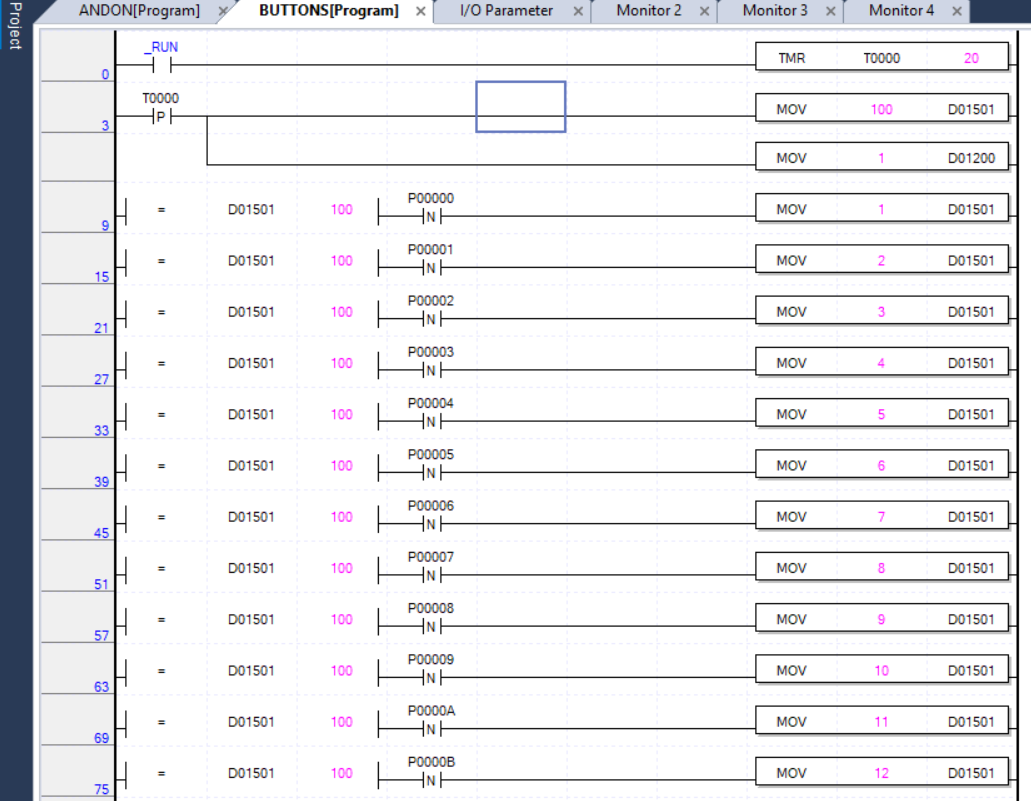
\includegraphics[width=0.72\textwidth]{Imagens/clp_04_buttons_inicializacao.png}
    \caption{BUTTONS: inicialização de \cod{D01501} em 100 e bordas de descida que selecionam os estados 1 a 12. (arquivo: Imagens/clp\_04\_buttons\_inicializacao.png)}
\end{figure}

\begin{figure}[H]
    \centering
    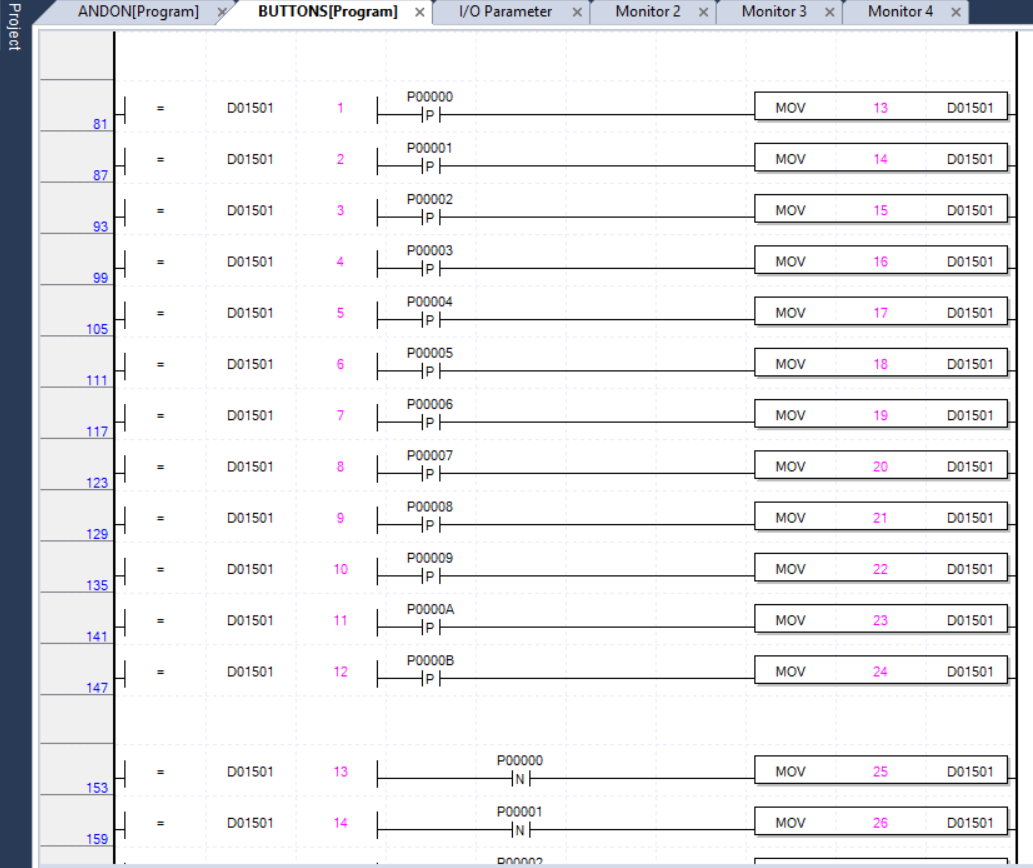
\includegraphics[width=0.72\textwidth]{Imagens/clp_05_buttons_borda_subida.png}
    \caption{BUTTONS: bordas de subida levam \cod{D01501} de 1-12 para 13-24. (arquivo: Imagens/clp\_05\_buttons\_borda\_subida.png)}
\end{figure}

\begin{figure}[H]
    \centering
    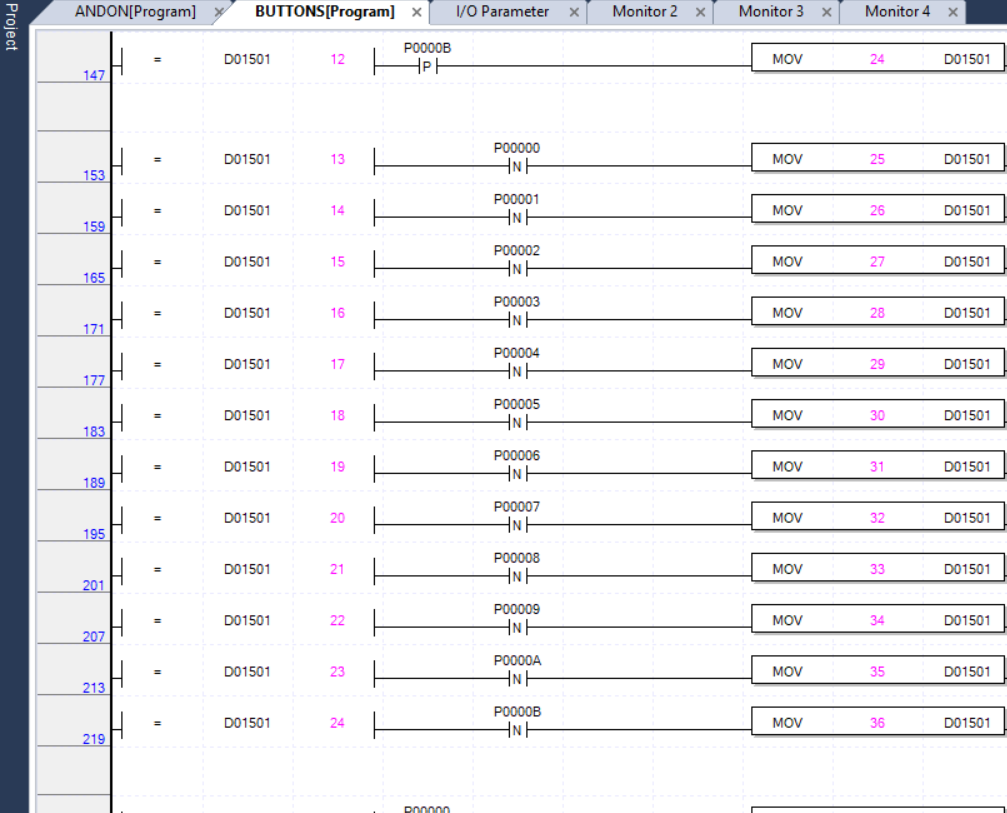
\includegraphics[width=0.72\textwidth]{Imagens/clp_06_buttons_borda_descida.png}
    \caption{BUTTONS: bordas de descida seguintes levam \cod{D01501} de 13-24 para 25-36. (arquivo: Imagens/clp\_06\_buttons\_borda\_descida.png)}
\end{figure}

\begin{figure}[H]
    \centering
    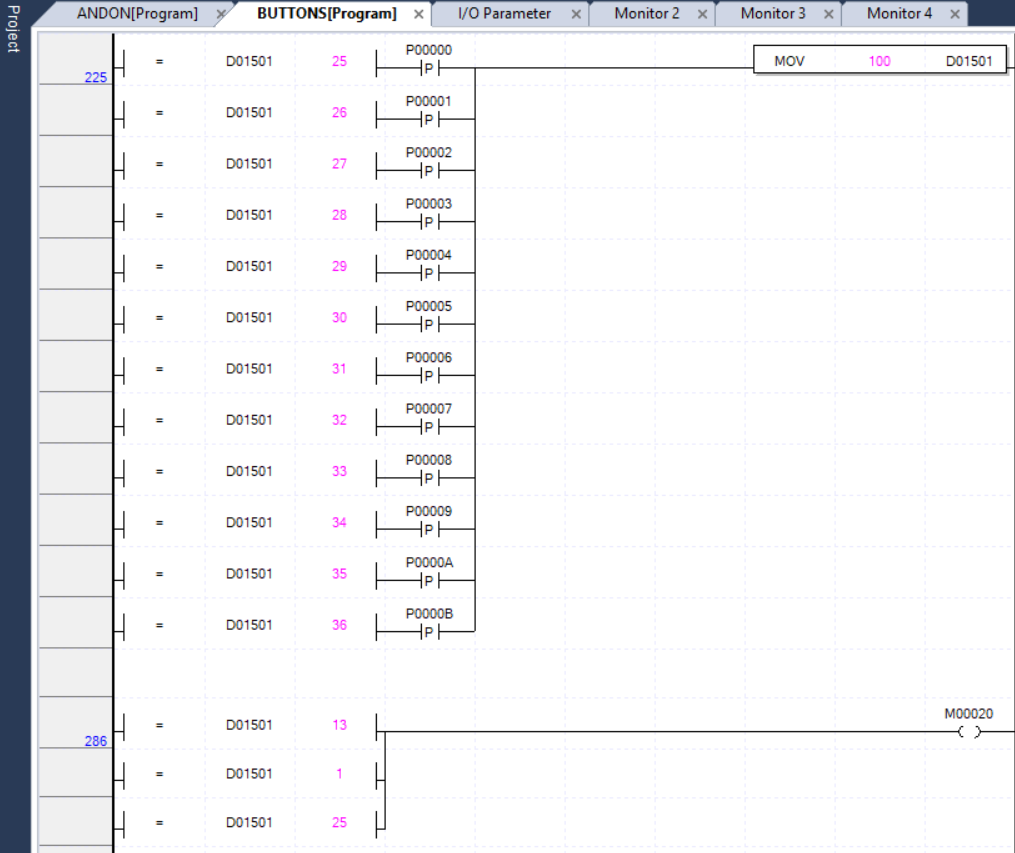
\includegraphics[width=0.72\textwidth]{Imagens/clp_07_buttons_retorno.png}
    \caption{BUTTONS: nos estados 25-36, a subida da entrada devolve \cod{D01501} a 100. (arquivo: Imagens/clp\_07\_buttons\_retorno.png)}
\end{figure}

\begin{figure}[H]
    \centering
    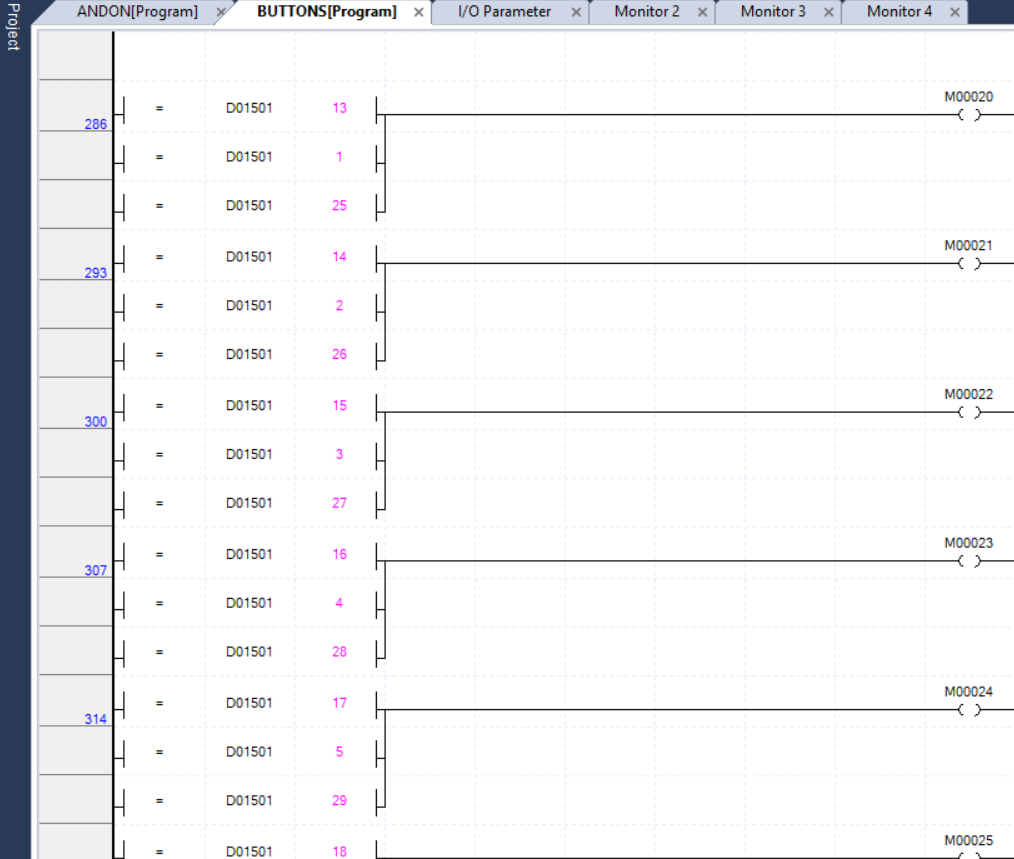
\includegraphics[width=0.72\textwidth]{Imagens/clp_08_buttons_marcas.png}
    \caption{BUTTONS: conversão dos estados em marcas; \cod{M00020} ativa em 1, 13 ou 25. (arquivo: Imagens/clp\_08\_buttons\_marcas.png)}
\end{figure}

\begin{figure}[H]
    \centering
    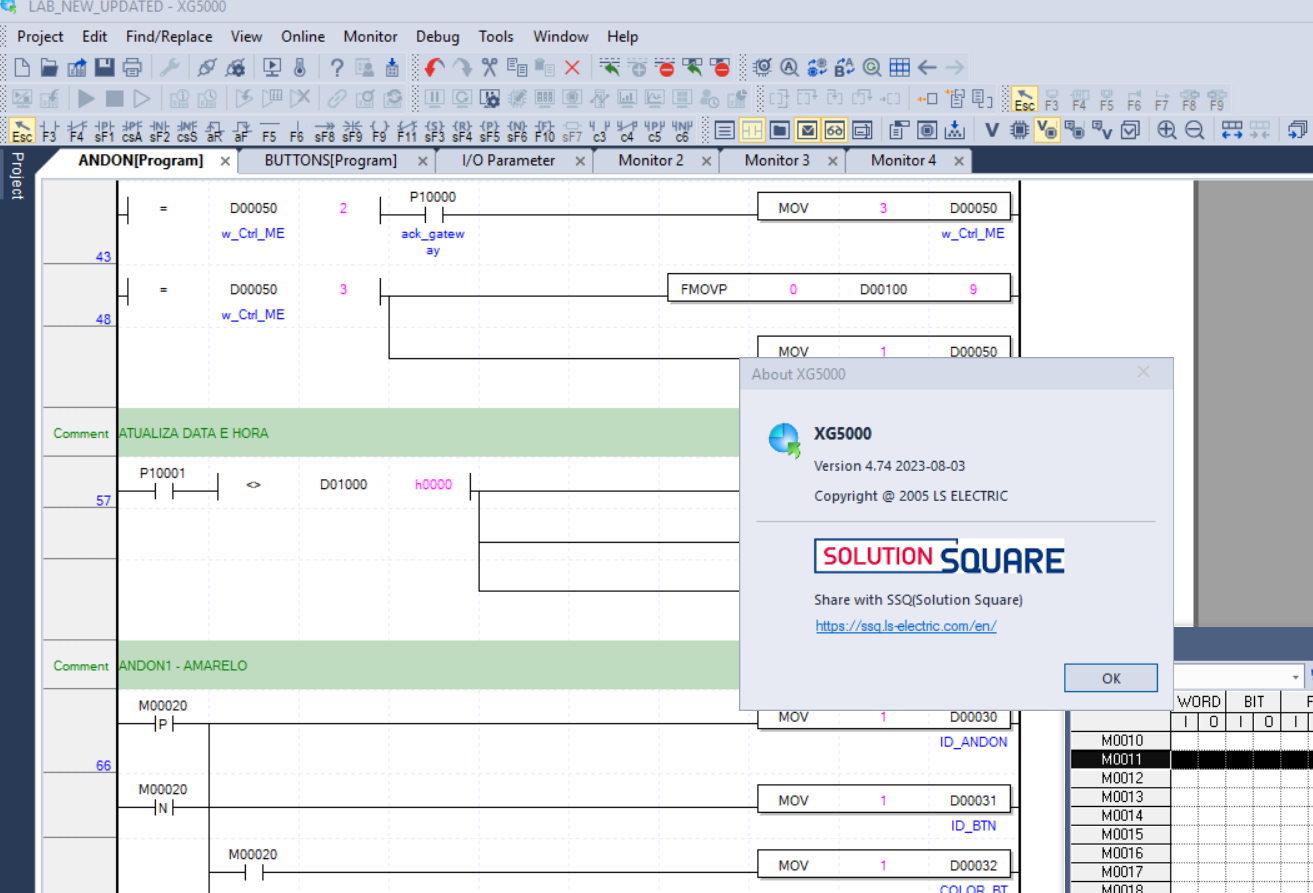
\includegraphics[width=0.72\textwidth]{Imagens/clp_03_versao_xg5000.png}
    \caption{Janela \textit{About XG5000}: versão 4.74. (arquivo: Imagens/clp\_03\_versao\_xg5000.png)}
\end{figure}

\begin{figure}[H]
    \centering
    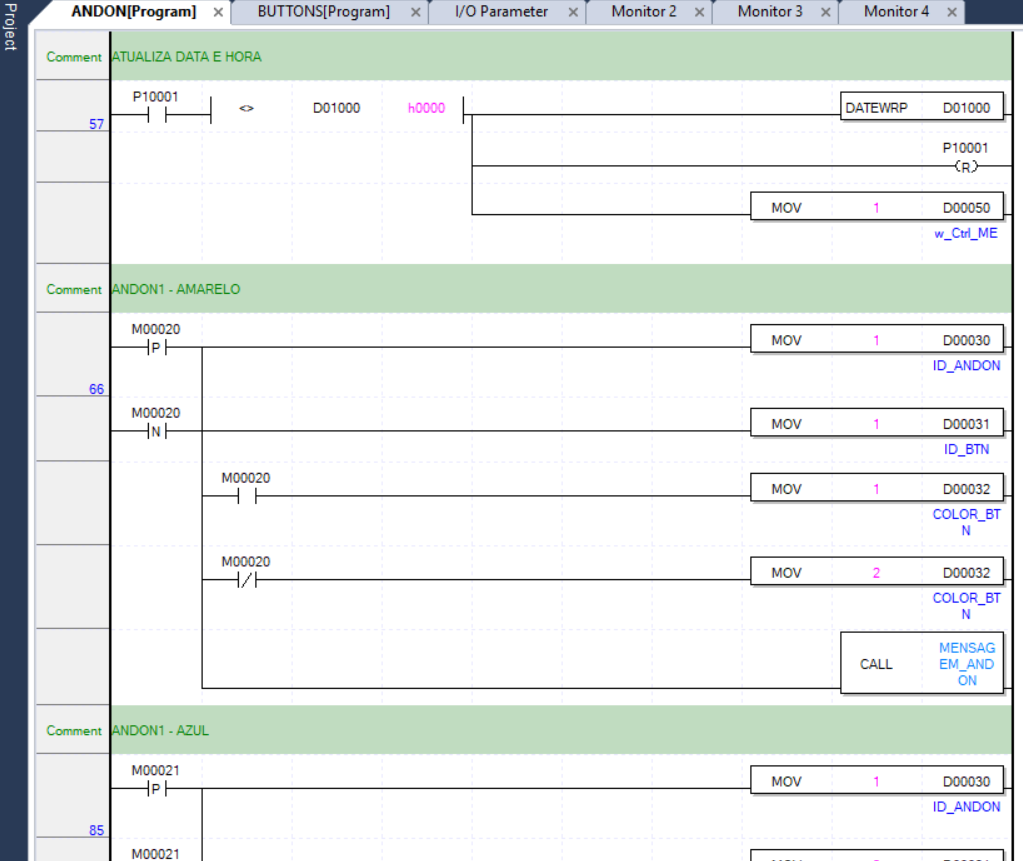
\includegraphics[width=0.72\textwidth]{Imagens/clp_11_andon_relogio_amarelo.png}
    \caption{ANDON: aplicação do relógio (\cod{P10001} e \cod{DATEWRP D01000}) e rede do Andon amarelo. (arquivo: Imagens/clp\_11\_andon\_relogio\_amarelo.png)}
\end{figure}

\begin{figure}[H]
    \centering
    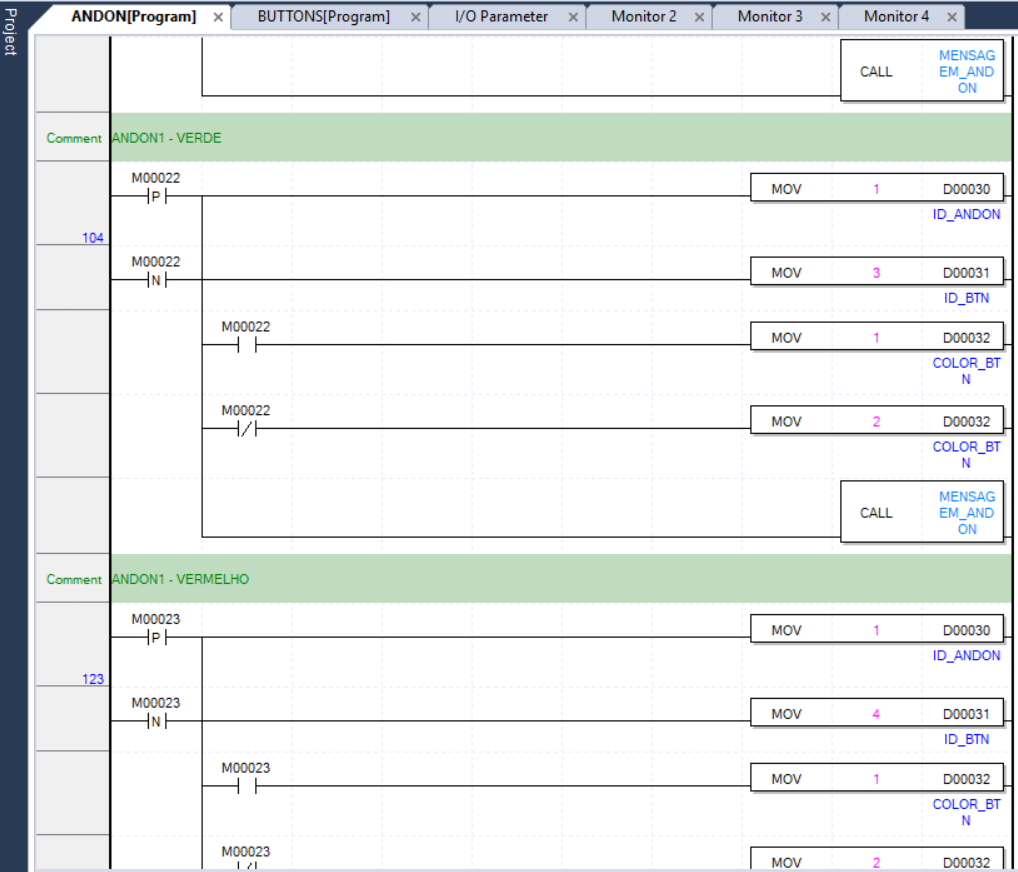
\includegraphics[width=0.72\textwidth]{Imagens/clp_12_andon_verde_vermelho.png}
    \caption{ANDON: redes dos Andons verde e vermelho. (arquivo: Imagens/clp\_12\_andon\_verde\_vermelho.png)}
\end{figure}

\begin{figure}[H]
    \centering
    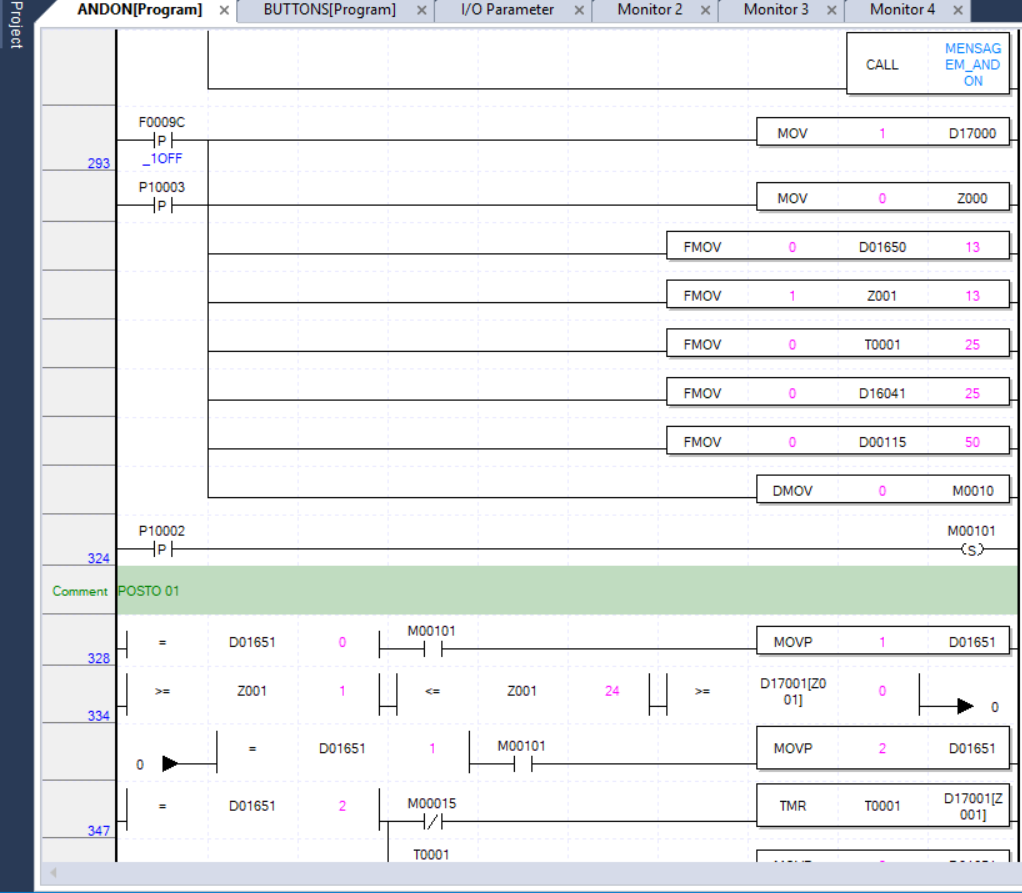
\includegraphics[width=0.72\textwidth]{Imagens/clp_14_inicializacao_start_reset.png}
    \caption{Redes de reset (\cod{P10003}) e Start (\cod{P10002} $\rightarrow$ \cod{M00101}). (arquivo: Imagens/clp\_14\_inicializacao\_start\_reset.png)}
\end{figure}

\begin{figure}[H]
    \centering
    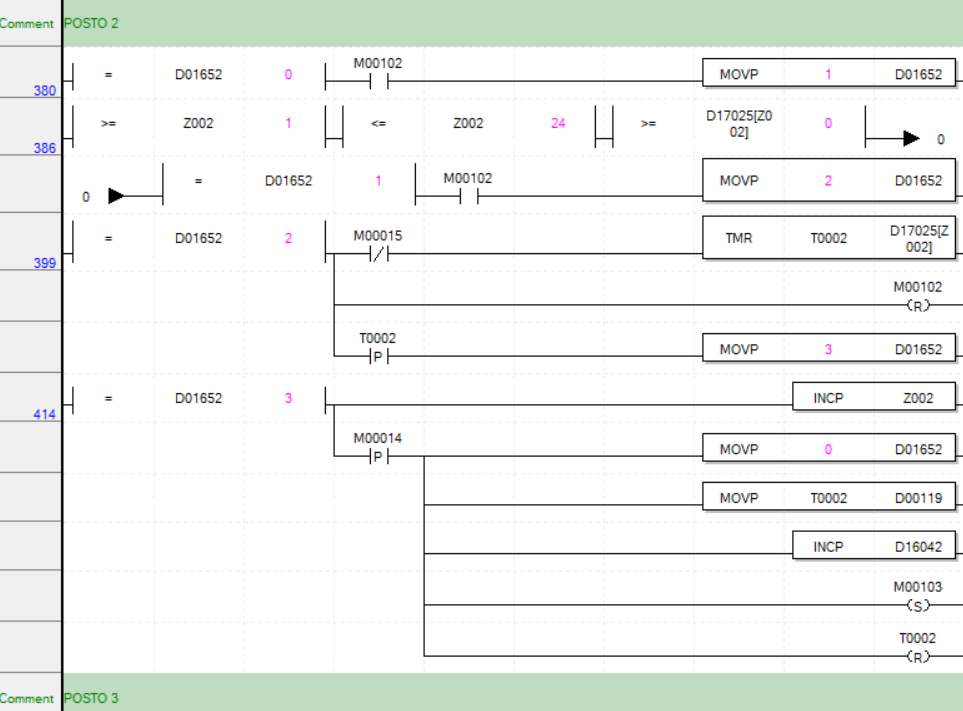
\includegraphics[width=0.72\textwidth]{Imagens/clp_16_posto_02.png}
    \caption{Posto 02: \cod{D01652}, \cod{T0002} e incremento de \cod{D16042}. (arquivo: Imagens/clp\_16\_posto\_02.png)}
\end{figure}

\begin{figure}[H]
    \centering
    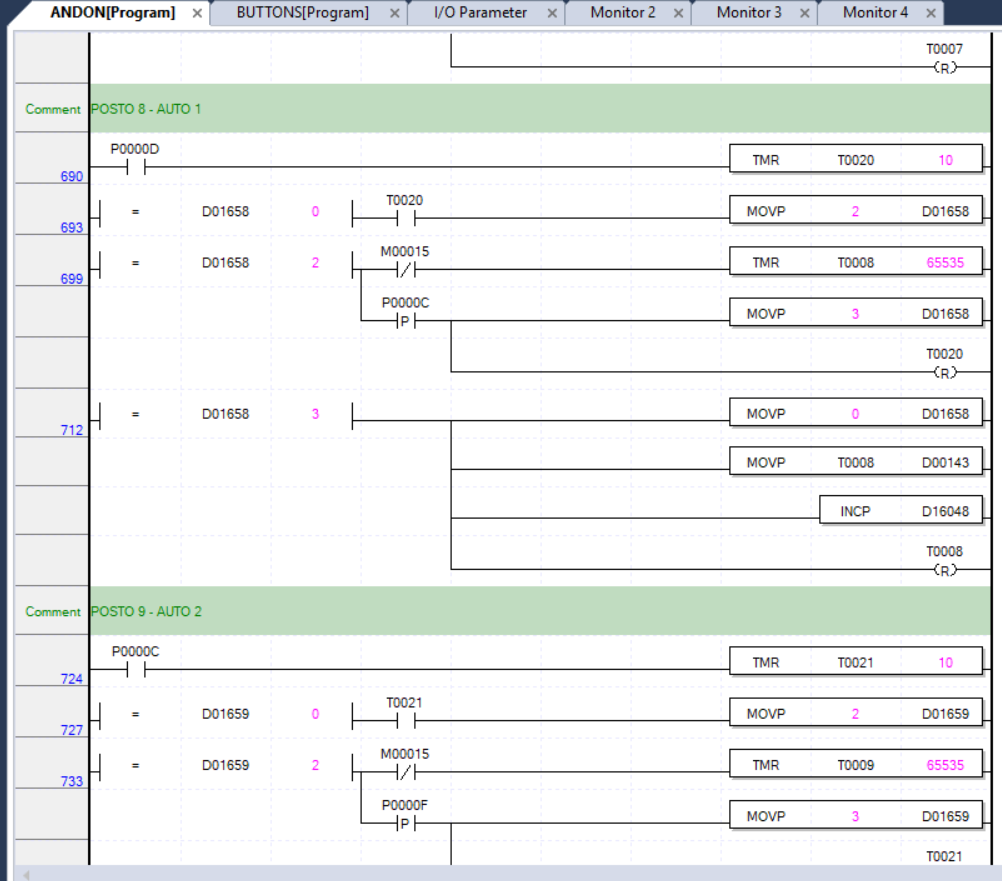
\includegraphics[width=0.72\textwidth]{Imagens/clp_18_posto_08_auto_1.png}
    \caption{Posto 08 (Auto 1): entrada por \cod{P0000D} e término pela borda de \cod{P0000C}. (arquivo: Imagens/clp\_18\_posto\_08\_auto\_1.png)}
\end{figure}

\begin{figure}[H]
    \centering
    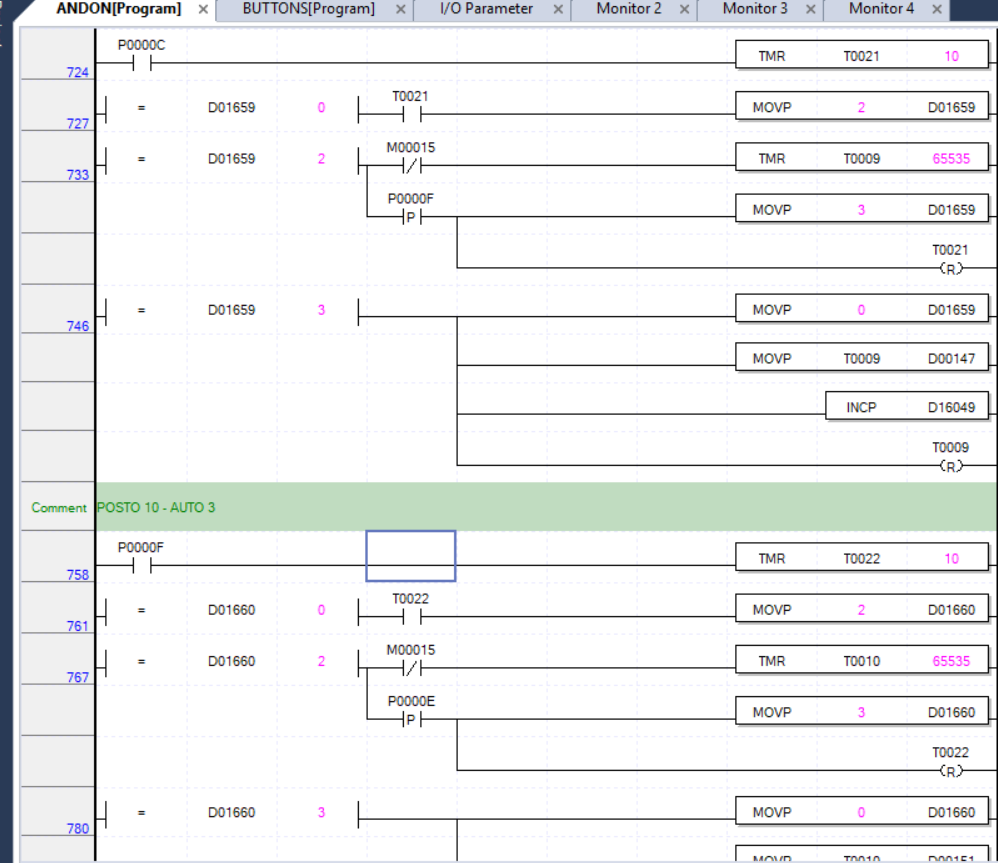
\includegraphics[width=0.72\textwidth]{Imagens/clp_19_posto_09_auto_2.png}
    \caption{Posto 09 (Auto 2): estado em \cod{D01659}; tempo de \cod{T0009} copiado para \cod{D00147}. (arquivo: Imagens/clp\_19\_posto\_09\_auto\_2.png)}
\end{figure}

\begin{figure}[H]
    \centering
    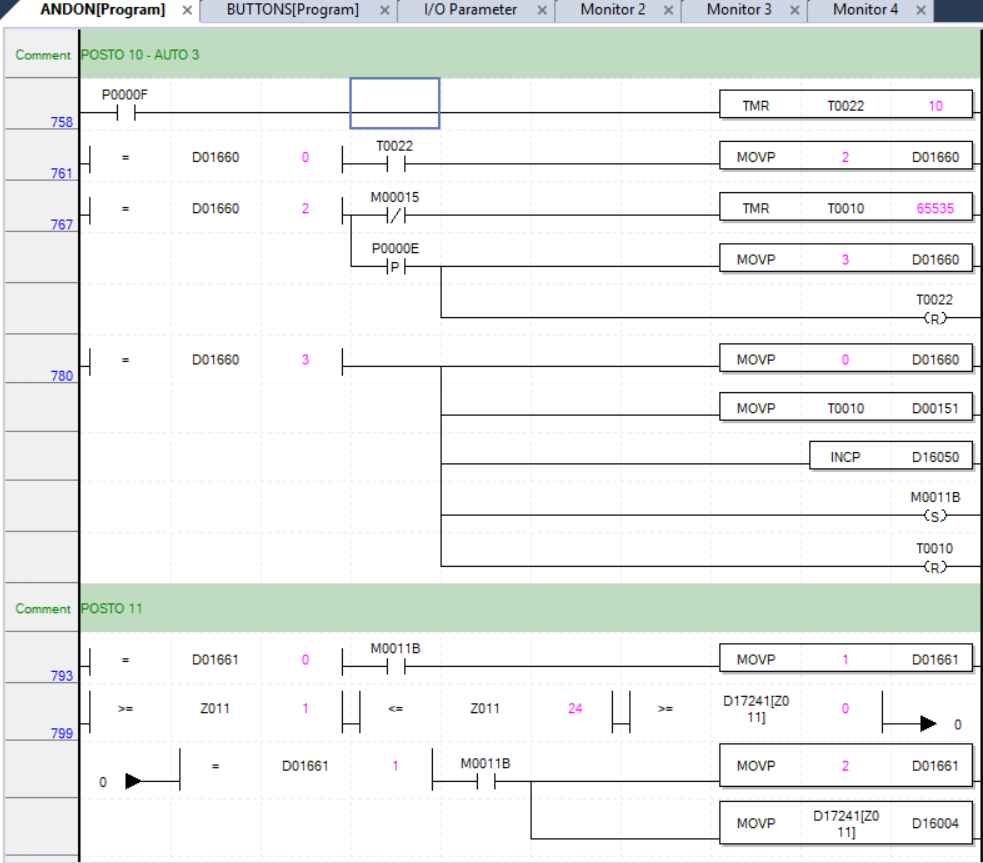
\includegraphics[width=0.72\textwidth]{Imagens/clp_20_posto_10_auto_3.png}
    \caption{Posto 10 (Auto 3): registro em \cod{D00151}, incremento de \cod{D16050} e sinal ao P11 por \cod{M0011B}. (arquivo: Imagens/clp\_20\_posto\_10\_auto\_3.png)}
\end{figure}
